%Todo poprwic niespojnosci: moduł View czy Scene?
\chapter {Projekt}
Głównym celem projektu jest stworzenie i weryfikacja modelu rozprzestrzeniania się ognia wykorzystując niehomogeniczne automaty
komórkowe, który został opisany w rozdziale \ref{cha:Algorytm} . Nacisk z pracy został położony na opracowanie algorytmu najdokładniej oddającego rzeczywistość.
Aplikacja, o nazwie Sparkle została zaprojektowana tak, aby zapewnić użytkownikowi wysoką ergonomię pracy i łatwość nauki.
Podczas projektowania i implementacji szczególna uwaga została poświęcona dalszym możliwościom rozbudowy programu oraz testowania 
kolejnych wersji modelu algorytmicznego. Wstęp poniższego rozdziału zawiera ogólne założenia dotyczącego całego projektu. 
Następni w kolejnych podrozdziałach została opisana architektura aplikacji oraz budowa i funkcjonowanie poszczególnych modułów.
\label{cha:projekt}
\section {Główne założenia}
\begin {itemize}
\item Projekt obejmuje zarówno stworzenie i weryfikację modelu rozprzestrzeniania pożaru jak i zaimplementowanie uproszczonej wizualizacji oraz graficznego interfejsu użytkownika (GUI).
\item Interfejs aplikacji powinien umożliwiać edycję budynku w którym przeprowadzana jest symulacja: dodawanie elementów konstrukcji, 
określanie materiałów z których zostały stworzone. 
\item Użytkownik powinien mieć możliwość określenia źródła ognia (miejsca w którym rozpoczyna się pożar).
\item Aplikacja powinna umożliwiać kontrolę nad symulacją: możliwość zatrzymania symulacji, wznowienia, rozpoczęcia od początku.
\item Dodatkowym elementem jest zapis wyników w postaci rozkładu temperatur do pliku, umożliwiający dogłębną analizę rezultatów.
\item Wizualizacja powinna obejmować zarówno rozkład temperaturowy jak i rozprzestrzenianie się rozprzestrzenianie ognia. 
\end {itemize}
\section {Architektura aplikacji}
Aplikacja została podzielona na trzy główne moduły:
\begin{itemize}
\item Controller - odpowiada za interakcję z użytkownikiem, dostarcza GUI umożliwiające kontrolę symulacji
\item Model - przechowuje model symulacji, realizuje algorytmy rozprzestrzeniania ognia
\item View - odpowiada za wizualizację wyników
\end{itemize}
Zależności pomiędzy poszczególnymi komponentami przedstawia diagram komponentów \ref{architektura aplikacji}
\begin{figure}
\begin {center}
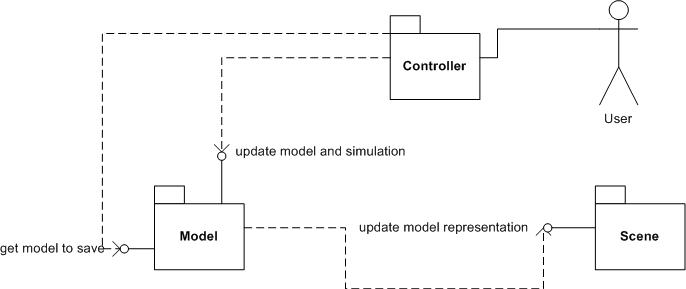
\includegraphics{architectureComponentDiagram.jpg} \\
\caption { Architektura aplikacji}
\label {architektura aplikacji}
\end {center}
\end{figure}
Zapewnienie bardzo prostych relacji między modułami pozwala niezależnie rozwijać kolejne części aplikacji, w łatwy
sposób podmieniać i modyfikować ich zachowanie. Inną zaletą zastosowanego modelu jest łatwość
testowania poszczególnych części programu niezależnie.

Przedstawiony model powstał na bazie jednego z najpopularniejszych modeli tworzenia aplikacji wykorzystujących graficzny interfejs użytkownika: Model-View-Controller. Elementem różniącym przedstawiony powyżej model od tradycyjnej architektury Model-View-Controller
jest rozdzielenie elementów GUI pomiędzy dwa moduły:
\begin{itemize}
\item Scene przedstawiającą wyniki aplikacji oraz
\item Controller, który łączy w sobie elementy kontroli i widoku dostarczając użytkownikowi zestaw narzędzi umożliwiających komunikację z aplikacją.
\end {itemize}
\subsection{Moduł Controller}
Moduł kontroler odpowiada za komunikację między użytkownikiem a silnikiem aplikacji (elementem realizującym logikę algorytmiczną). 
Jego podstawowym zadaniem jest dostarczenie łatwego w obsłudze, graficznego interfejsu oraz 
obsługa akcji użytkownika. Wspomniana obsługa akcji obejmuje zarówno zebranie danych od użytkownika, ich przetworzenie
i dostarczenie do modelu jak i pobranie z modelu danych i ich eksport na zewnątrz aplikacji.
Funkcjonalności dostarczane przez moduł Controller przedstawia diagram przypadków użycia \ref{przypadki uzycia}.
\begin{figure}
\begin {center}
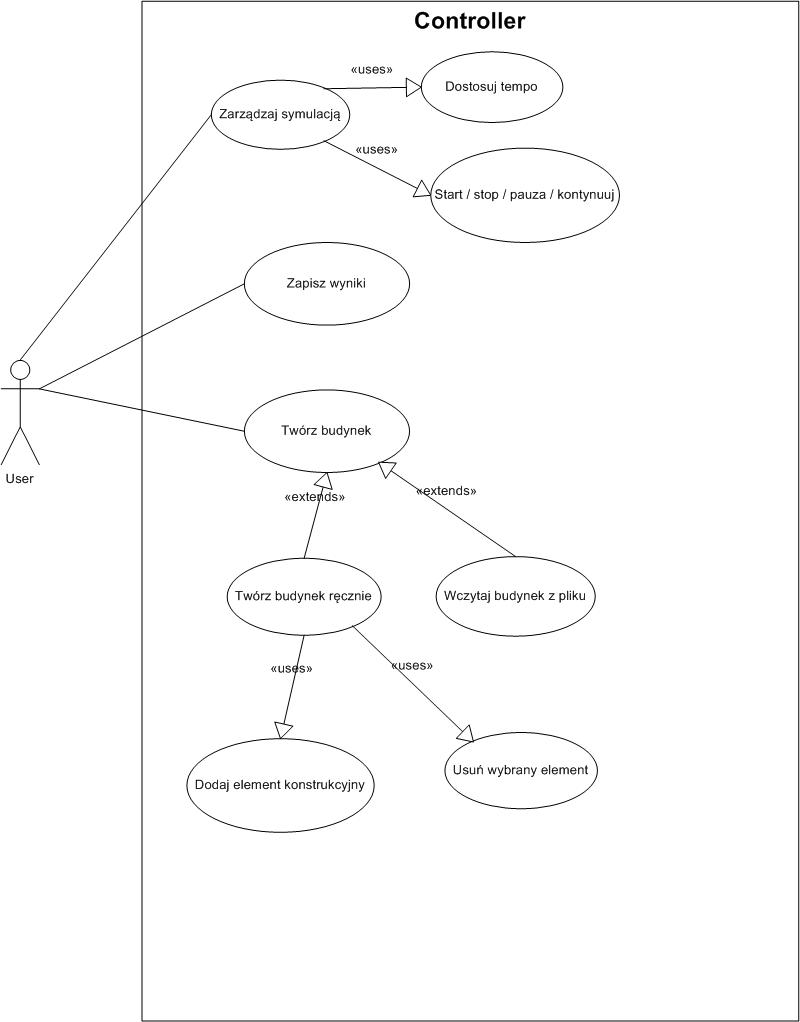
\includegraphics{useCase.jpg} \\
\caption { Przypadki użycia}
\label {przypadki uzycia}
\end {center}
\end{figure}


Controller zbudowany jest z następujących klas.
\begin{itemize}
\item Editor - dostarcza użytkownikowi pole tekstowe umożliwiające edycję budynku. Rejestruje obiekty nasłuchujące, w dalszym ciągu tekstu nazywane Listenerami, których zadaniem jest przechwytywanie akcji i ich obsługa w ramach metod zwanych Handlerami. W przypadku edytora nasłuchiwanie ogranicza się do komend wprowadzanych z klawiatury. Tekst wprowadzony do edytora jest przekazywany klasie EditorParser do dalszego przetworzenia.
\item EditorParser - odpowiada za parsowanie, czyli analizę otrzymanego tekstu oraz wywołanie odpowiednich metod modelu odpowiadających za 
dodanie / usunięcie bloku.
\item MainWindow - reprezentuje główne okno aplikacji. Zawiera edytor tekstowy, scenę, na której przedstawiane są wyniki symulacji oraz 
zestaw paneli menu. Odpowiada za rozmiary i rozmieszczenie zawieranych elementów.
\item MenuPanel - dostarcza zestaw narzędzi (guzików, pól tekstowych, opcji wyboru) umożliwiających sterowanie aplikacją, dodawanie bloków do budynku oraz przeglądanie tekstu pomocy. Rejestruje Listenery obsługujące wyżej wymienione akcje.
\item TopMenu - zawiera elementy umożliwiające zapis wyników symulacji do pliku oraz wprowadzenie budynku z pliku.
\item FileChooser - okno wyboru pliku z którego następuje odczyt parametrów budynku lub do którego zapisywane są wyniki.
\item SimulationMgr - odpowiada za przebieg symulacji. Reguluje jej tempo, obsługuje zdarzenia wstrzymania / wznowienia.
\end {itemize}

\subsection {Moduł View}
Jedynym zadaniem widoku, zwanego dalej także sceną jest graficzne przedstawienie dostarczonego modelu.
Moduł View nie korzysta z żadnych innych modułów.
Całkowite odizolowanie widoku od innych komponentów umożliwia jego łatwą modyfikację. Pakiet Scene zawiera klasę
\begin {itemize}
\item Scene3D - odpowiedzialną za wizualizację stworzonego budynku oraz aktualizację widoku podczas symulacji.
\end {itemize}
\subsection {Moduł Model}
Komponent model jest silnikiem aplikacji. Zawiera struktury danych oraz algorytmy realizujące symulację w oparciu o niehomogeniczny automat komórkowy. Składa się z następujących klas:
\begin {itemize}
\item Cell - zawiera zestaw atrybutów opisujących pojedynczą komórkę automatu oraz metod umożliwiających dostęp do nich. Do atrybutów komórki należą:
\begin {itemize}
\item Materiał
\item Masa
\item Temperatura
\item Stan
\item Zawartość palnych oparów
\item Czas pozostały do całkowitego spalenia komórki
\end {itemize}
\item Material - opisuje właściwości materiału z którego może być zbudowana komórka.
Do właściwości materiału należą:
\begin {itemize}
\item Nazwa
\item Kolor
\item Przeźroczystość
\item Czas spalania
\item Ciepło właściwe
\item Przewodnictwo ciepła
\item Temperatura zapłonu
\item Palność - wartość określająca czy materiał jest paliwem czy nie.
\end {itemize}
\item HeatCondctor - odpowiada za obliczenie ilości energii przekazanej za pomocą przewodnictwa między komórkami. Uaktualnia temperaturę komórek w wyniku przekazania energii.  
\item HeatAndVaporsConductorWithConvection - odpowiada za obliczenie ilości energii przekazanej przez konwekcję. Uaktualnia temperaturę komórek w wyniku przekazania energii. Symuluje przepływ oparów, przenoszonych przez prądy konwekcyjne.
\item FireConductor - odpowiada za aktualizację stanu komórki
\item World - odpowiada za stworzenie modelu automatu odzwierciedlającego zbudowany obiekt. Aktualizuje stan automatu przez wywołanie metod klas HeatConducter, HeatAndVaporsConductorWithConvection, FireConductor.
\end {itemize}
Dokładną ilustrację zależności między klasami wchodzącymi w skład omówionych komponentów, z uwzględnieniem elementów implementacyjnych zawierają diagramy zamieszczone w rozdziale \ref{cha:implementacja}. %żeby od razu zawrzeć tam. ze np jakaś klasa dziedziczy po Composite czy użycie swinga itd.
 
